%!TEX root = ..\hdf5-structure.tex

\definecolor{mycolor1}{rgb}{0.9,0.9,0.9}%
\definecolor{mycolor2}{rgb}{0.65,0.65,0.65}%

\begin{forest}
	for tree={draw,
		edge path={
			\noexpand\path[\forestoption{edge}] (\forestOve{\forestove{@parent}}{name}.parent anchor) -- +(0,-8pt)-| (\forestove{name}.child anchor)\forestoption{edge label};
		}
	},
	A/.style={fill=mycolor1}, %style for attributes
	D/.style={fill=mycolor2}, %style for datasets
	G/.style={}, %style for groups
	[/
		[/version, A]
		[/background, G
			[/1, D
				[/date, A]
			]
		]
		[/payload, G
			[/resolution-x, A]
			[/resolution-y, A]
			[/data, G, l=2.47cm,before computing xy={s=2.85cm}
				[/1, D
					[/date, A]
				]
				[/..., D
					[/date, A]
				]
				[/$N$, D
					[/date, A]
				]
			]
			[/positions-x, D]
			[/positions-y, D]
		]
		[/date, A]
		[/comments, A]
  ]
\end{forest}
\vspace{5mm}\\
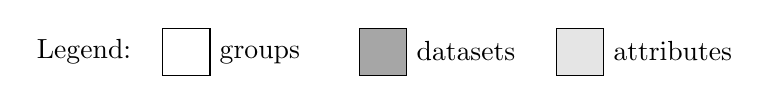
\begin{tikzpicture}
\node at (0,0) {Legend:};

\draw [] (1.0,-0.3) -- ++(0.6,0) -- ++(0,0.6) -- ++(-0.6,0) -- cycle;
\node [anchor=west,align=left,text height=1.5ex]at (1.6,0.0) {groups};

\draw [fill=mycolor2] (3.5,-0.3) -- ++(0.6,0) -- ++(0,0.6) -- ++(-0.6,0) -- cycle;
\node [anchor=west,align=left,text height=1.5ex]at (4.1,0.0) {datasets};

\draw [fill=mycolor1] (6.0,-0.3) -- ++(0.6,0) -- ++(0,0.6) -- ++(-0.6,0) -- cycle;
\node [anchor=west,align=left,text height=1.5ex]at (6.6,0.0) {attributes};
\end{tikzpicture}